\documentclass[aspectratio=169, table]{beamer}

\usepackage[utf8]{inputenc}
\usepackage{listings} 

\usetheme{Pradita}

\subtitle{IF140303-Web Application Development}

\title{Session-01:\\
\vspace{10pt}
\Huge{Introduction to Elixir}
%\vspace{5pt}
}

\date[Serial]{\\\vspace{15pt}\scriptsize {PRU/SPMI/FR-BM-18/0222}}
\author[Pradita]{\small{\textbf{Alfa Yohannis}}}

\lstdefinelanguage{Elixir} {
	keywords={def, defmodule, do, end, for, if, else, true, false},
	basicstyle=\ttfamily\small,
	keywordstyle=\color{blue}\bfseries,
	ndkeywords={@moduledoc, iex, Enum, @doc},
	ndkeywordstyle=\color{purple}\bfseries,
	sensitive=true,
	numbers=left,
	numberstyle=\tiny\color{gray},
	breaklines=true,
	frame=lines,
	backgroundcolor=\color{lightgray!10},
	tabsize=2,
	comment=[l]{\#},
	morecomment=[s]{/*}{*/},
	commentstyle=\color{gray}\ttfamily,
	showstringspaces=false,
	% string settings
	morestring=[b]",
	morestring=[b]',
	stringstyle=\color{black}\ttfamily, % default, will be overridden
	moredelim=[s][\color{blue}\ttfamily]{"}{"},   % double quotes
	moredelim=[s][\color{teal}\ttfamily]{'}{'}    % single quotes
}


\lstdefinelanguage{bash} {
	keywords={},
	basicstyle=\ttfamily\small,
	keywordstyle=\color{blue}\bfseries,
	ndkeywords={iex},
	ndkeywordstyle=\color{purple}\bfseries,
	sensitive=true,
	commentstyle=\color{gray},
	stringstyle=\color{red},
	numbers=left,
	numberstyle=\tiny\color{gray},
	breaklines=true,
	frame=lines,
	backgroundcolor=\color{lightgray!10},
	tabsize=2,
	comment=[l]{\#},
	morecomment=[s]{/*}{*/},
	commentstyle=\color{gray}\ttfamily,
	stringstyle=\color{purple}\ttfamily,
	showstringspaces=false
}

\begin{document}
	
	\frame{\titlepage}


	\begin{frame}[fragile]
		\frametitle{Contents}
		\vspace{20pt}
		\begin{columns}[t]
			\column{0.5\textwidth}
			\tableofcontents[sections={1-5}]
			
			\column{0.5\textwidth}
			\tableofcontents[sections={6-20}]
		\end{columns}
	\end{frame}

\section{About Elixir}

\begin{frame}{Why Elixir Exists}
	\vspace{20pt}
	\begin{itemize}
		\item \textbf{Overcoming Limitations.} Elixir was designed to solve scalability, reliability, and concurrency issues often found in traditional programming languages.  
		\item \textbf{Built on BEAM.} Running on the Erlang Virtual Machine (BEAM, Bogdan/Björn’s Erlang Abstract Machine), Elixir inherits proven features such as fault tolerance, distribution, and massive concurrency.  
		\item \textbf{Developer Productivity.} Clean syntax, metaprogramming, and expressive design make coding faster, clearer, and easier to maintain.  
		\item \textbf{Modern Web Support.} With Phoenix, Elixir enables real-time communication and scalable, interactive web applications suitable for today’s demands.  
	\end{itemize}
\end{frame}

\subsection{Sejarah Elixir}

\begin{frame}{History of Elixir}
	\vspace{20pt}
	\begin{itemize}
		\item \textbf{2011.} José Valim introduced Elixir as an open-source project, aiming to combine Erlang’s scalability and fault tolerance with modern syntax.  
		\item \textbf{2014.} Version 1.0 was released, marking stability and readiness for production use, with robust features and integration support.  
		\item \textbf{2015.} The Phoenix web framework launched, enabling real-time, dynamic web applications with LiveView and advanced tooling.  
		\item \textbf{2018.} Adoption expanded across industries like fintech and telecom, supported by an active community and growing ecosystem.  
		\item \textbf{2021+.} Elixir continues to evolve with better tooling, libraries, and support for modern technologies.  
	\end{itemize}
\end{frame}

\subsection{Keunggulan Elixir}

\begin{frame}{Strengths of Elixir}
	\vspace{20pt}
	\begin{itemize}
		\item \textbf{Concurrency and Parallelism.} Lightweight processes communicate via message passing, enabling applications to efficiently manage thousands of concurrent tasks.  
		\item \textbf{Fault Tolerance.} Following Erlang’s “let it crash” philosophy with supervision trees, systems remain reliable even when individual components fail.  
		\item \textbf{Scalability.} Supports both vertical and horizontal scaling across distributed nodes, handling increasing workloads with ease.  
		\item \textbf{Metaprogramming.} Developers can generate code at compile time, build DSLs, and extend the language flexibly.  
		\item \textbf{Web Development.} Phoenix framework provides real-time communication, distributed components, and tools for responsive web applications.  
	\end{itemize}
\end{frame}

\subsection{Kelemahan Elixir}

\begin{frame}{Weaknesses of Elixir}
	\vspace{20pt}
	\begin{itemize}
		\item \textbf{Learning Curve.} Developers unfamiliar with functional programming or Erlang may struggle with concepts like immutability, recursion, and concurrency models.  
		\item \textbf{Limited Ecosystem.} While growing, Elixir still lacks the extensive libraries and third-party integrations found in JavaScript or Python.  
		\item \textbf{CPU-Intensive Tasks.} Elixir excels at concurrency and I/O-bound work but performs less efficiently in heavy computations or complex algorithms.  
		\item \textbf{Community and Documentation.} Resources are smaller compared to more popular languages, posing challenges for beginners seeking guidance.  
		\item \textbf{Legacy Integration.} Connecting Elixir with older systems often requires extra effort in compatibility and maintenance.  
	\end{itemize}
\end{frame}

\section{Installation and Project}

\begin{frame}[fragile]{Installing Elixir with Homebrew}
	\vspace{20pt}
	\begin{itemize}
		\item \textbf{Unified Installation.} The easiest way to install Elixir across macOS, Linux (including Ubuntu), and Windows (via WSL or Homebrew for Windows) is by using Homebrew.  
		\item \textbf{Install Homebrew.} If not already installed, follow the instructions at \url{https://brew.sh/}.  
		\item \textbf{Install Elixir.} Once Homebrew is available, run the following command in your terminal:
	\end{itemize}
	
	\begin{lstlisting}[language=bash]
		brew install elixir
	\end{lstlisting}
	
	\begin{itemize}
		\item \textbf{Verify Installation.} Confirm Elixir is ready by checking its version:
	\end{itemize}
	
	\begin{lstlisting}[language=bash]
		elixir --version
	\end{lstlisting}
\end{frame}


\begin{frame}[fragile]{Elixir Project in VS Code}
	\vspace{20pt}
	\begin{itemize}
		\item \textbf{Create Project.} Open a terminal, navigate to your chosen directory, and run:
	\end{itemize}
	
	\begin{lstlisting}[language=bash]
		mix new project_name
		cd project_name
	\end{lstlisting}
	
	\begin{itemize}
		\item \textbf{Open in VS Code.} Launch VS Code, select \texttt{File > Open Folder}, and choose the new project. Alternatively, run:
	\end{itemize}
	
	\begin{lstlisting}[language=bash]
		code .
	\end{lstlisting}
	
	\begin{itemize}
		\item \textbf{Install Plugin.} From the VS Code Marketplace, install \textbf{ElixirLS: Elixir support and debugger} to enable syntax highlighting, IntelliSense, debugging, and test integration.
		\item \textbf{Start Coding.} With the plugin active and project open, you are ready to develop Elixir applications.
	\end{itemize}
\end{frame}


\section{Object-oriented vs Functional Programming}

\begin{frame}{Object-Oriented Programming (OOP)}
	\vspace{20pt}
	\begin{itemize}
		\item \textbf{Definition.} OOP emphasizes creating objects that represent real-world entities, combining attributes (data) and methods (functions).  
		\item \textbf{Mutable State.} Objects can change their state during execution, e.g., methods modify attribute values.  
		\item \textbf{Key Concepts.}
		\begin{itemize}
			\item \textbf{Classes and Objects:} Blueprint and its instances.  
			\item \textbf{Encapsulation:} Bundling data and methods for controlled access.  
			\item \textbf{Inheritance:} Building new classes from existing ones.  
			\item \textbf{Polymorphism:} One interface, multiple implementations.  
		\end{itemize}
	\end{itemize}
\end{frame}

\begin{frame}{OOP Illustration}
	\vspace{10pt}
	\begin{columns}[]
		\column{0.35\textwidth}
		\textbf{Explanation.}  
		The method \texttt{generate\_pool} initializes \texttt{coupons} in object \texttt{lottery1},  
		while \texttt{randomize} modifies the state of \texttt{coupons}.  
		
		\vspace{10pt}
		This illustrates how objects in OOP can mutate their internal state  
		through methods that operate directly on their attributes.
		
		\column{0.65\textwidth}
		\centering
		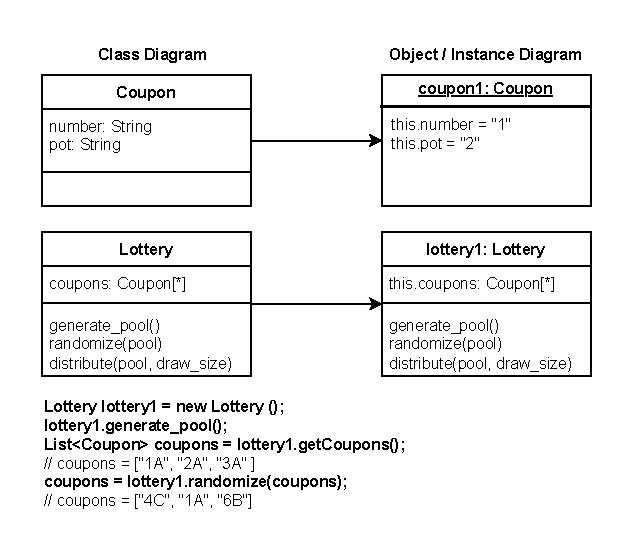
\includegraphics[width=\textwidth]{../../assets/object-oriented.pdf}
	\end{columns}
\end{frame}

\begin{frame}{Functional Programming (FP)}
	\vspace{20pt}
	\begin{itemize}
		\item \textbf{Definition.} FP is based on mathematical functions without side effects, always returning the same result for identical input.  
		\item \textbf{Immutable Data.} State is never changed directly; each operation produces a new copy of data (e.g., \texttt{copy list} then \texttt{randomize list}).  
		\item \textbf{Pure Functions.} Functions do not alter external state and are predictable in behavior.  
		\item \textbf{Recursion.} Iteration is achieved by self-calling functions instead of imperative loops.  
		\item \textbf{First-Class Functions.} Functions can be passed, returned, and stored like values.  
	\end{itemize}
\end{frame}

\begin{frame}{FP Illustration}
	\vspace{20pt}
	\begin{columns}
		\column{0.45\textwidth}
		\textbf{Explanation.}  
		In functional programming, data is immutable.  
		For example, \texttt{coupons = [A, B, C]} is first duplicated  
		(\texttt{copy list}), then randomized (\texttt{randomize list})  
		to produce \texttt{coupons = [C, A, B]}.  
		
		\vspace{10pt}
		This demonstrates that FP transformations return new data  
		rather than mutating the existing state.  
		
		\column{0.55\textwidth}
		\centering
		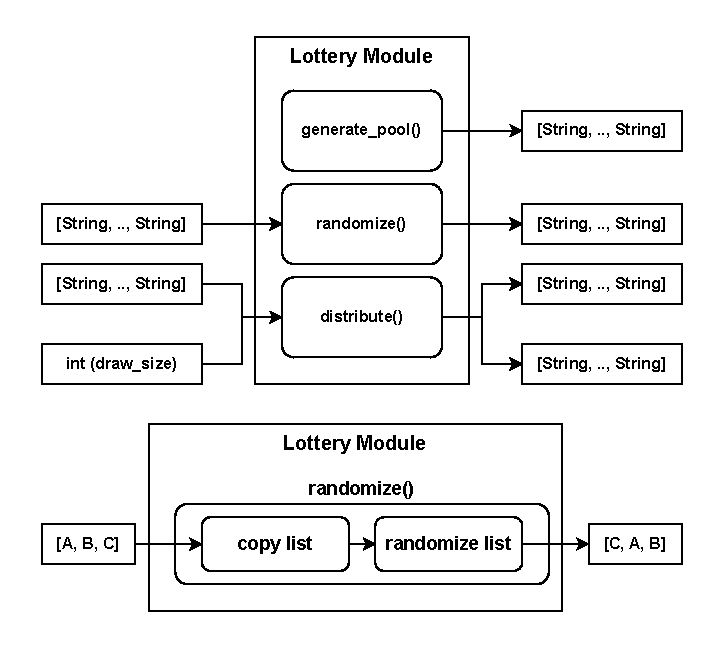
\includegraphics[width=\textwidth]{../../assets/functional.pdf}
	\end{columns}
\end{frame}

\begin{frame}{Comparison: OOP vs FP}
	\vspace{20pt}
	\begin{itemize}
		\item \textbf{State Management.} OOP emphasizes objects that store and mutate state through methods, while FP relies on pure functions that avoid mutation and instead return new transformed copies of data.  
		\item \textbf{Mutability vs Immutability.} In OOP, mutable state changes are common; in FP, data is immutable and modifications are expressed by creating new versions.  
		\item \textbf{Iteration.} OOP typically uses imperative loops; FP uses recursion and higher-order functions like \texttt{map}, \texttt{filter}, and \texttt{reduce}.  
		\item \textbf{Use Cases.} OOP suits interactive systems (e.g., GUIs, games), while FP is efficient for mathematical computation and data processing.  
	\end{itemize}
\end{frame}

\section{IEx (Repeat-Evaluate-Print-Loop)}
\begin{frame}[fragile]{Run and Test Elixir Code with IEx}
	\vspace{20pt}
\begin{columns}[t]
\column[t]{0.5\textwidth}
\textbf{About REPL.}  
IEx is Elixir’s REPL (\textit{Read–Eval–Print Loop}),  
an interactive environment to quickly test expressions,  
explore functions, and debug code.  

\begin{lstlisting}[language=Elixir]
$ iex
Interactive Elixir (1.16.0)
iex(1)>

iex(1)> 1 + 2 * 3
7

iex(2)> String.upcase("hello world")
"HELLO WORLD"
\end{lstlisting}

\column[t]{0.5\textwidth}
\begin{lstlisting}[language=Elixir]
# hello.exs
defmodule Hello do
def greet(name) do
"Hello, #{name}!"
end
end

iex(1)> c("hello.exs")
[Hello]

iex(2)> Hello.greet("Alice")
"Hello, Alice!"
\end{lstlisting}
\end{columns}
\end{frame}

\section{Elixir Project}

\begin{frame}[fragile]{Create \& Run an Elixir Project with Mix}
\vspace{20pt}
\begin{lstlisting}[language=Elixir]
$ mix new project_name
$ cd project_name
$ iex -S mix
\end{lstlisting}

\begin{itemize}
\item \textbf{Create Project.} \texttt{mix new} generates a new Elixir project with a standard structure.  
\item \textbf{Enter Directory.} Move into the project folder before running further commands.  
\item \textbf{Run in IEx.} \texttt{iex -S mix} starts IEx and loads the project so modules and dependencies are instantly available.  
\end{itemize}
\end{frame}


\begin{frame}[fragile]{Creating and Running Hello Project}
\begin{columns}[t]
\column{0.5\textwidth}
\begin{lstlisting}[language=Elixir]
$ mix new project_name
$ cd project_name

# lib/hello.ex
defmodule Hello do
	def greet(name) do
		"Hello, #{name}!"
	end
end
\end{lstlisting}

\column{0.5\textwidth}
\begin{lstlisting}[language=Elixir]
$ iex -S mix
Interactive Elixir (1.16.0)

iex(1)> Hello.greet("Alice")
"Hello, Alice!"
\end{lstlisting}

\textbf{Steps:}
\begin{itemize}
\item Create project with Mix.
\item Add \texttt{Hello} module in \texttt{lib/}.
\item Run with \texttt{iex -S mix}.
\item Test function in IEx.
\end{itemize}
\end{columns}
\end{frame}

\section{\texttt{String} Operations}

\begin{frame}[fragile]{Basic String Operations in Elixir}
\begin{columns}[t]
\column{0.5\textwidth}
\begin{lstlisting}[language=Elixir]
# Concatenate strings
greeting = "Hello, " <> "world!"
IO.puts(greeting)

# String interpolation
name = "Elixir"
message = "Welcome to #{name} programming!"
IO.puts(message)
\end{lstlisting}

\column{0.5\textwidth}
\begin{lstlisting}[language=Elixir]
# String length
len = String.length("Hello")
IO.puts(len)

# Uppercase
IO.puts(String.upcase("elixir"))

# Lowercase
IO.puts(String.downcase("ELIXIR"))
\end{lstlisting}

\vspace{8pt}

\end{columns}
\textbf{Explanation.}  
Strings can be concatenated, interpolated,  
measured, and converted to upper/lower case.  
These are the most common basic operations in Elixir.
\end{frame}


\section{\texttt{List} operations}

\begin{frame}[fragile]{Basic List Operations in Elixir}
\begin{columns}[t]
\column{0.5\textwidth}
\begin{lstlisting}[language=Elixir, basicstyle=\ttfamily\small]
# Create a list
list = [1, 2, 3, 4, 5]
IO.inspect(list)
# [1, 2, 3, 4, 5]

# Add element at head
new_list = [0 | list]
IO.inspect(new_list)
# [0, 1, 2, 3, 4, 5]
\end{lstlisting}

\vspace{6pt}
\textbf{Summary.}  
Lists can be created, concatenated,  
pattern matched, measured, and searched.  

\column{0.5\textwidth}
\begin{lstlisting}[language=Elixir, basicstyle=\ttfamily\small]
# Pattern matching
[head | tail] = list
IO.puts("Head: #{head}")
# Head: 1
IO.inspect(tail)
# [2, 3, 4, 5]

# Length
IO.puts("Length: #{length(list)}")
# Length: 5

# Membership
IO.puts(Enum.member?(list, 3))
# true
\end{lstlisting}
\end{columns}
\end{frame}

\section{\texttt{Enum} Module}

\begin{frame}[fragile]{Enum Module in Elixir}
\begin{columns}[t]
\column{0.5\textwidth}
\begin{lstlisting}[language=Elixir, basicstyle=\ttfamily\scriptsize]
# Shuffle
list = [1, 2, 3, 4, 5]
IO.inspect(Enum.shuffle(list))
# e.g. [3, 1, 4, 5, 2]

# Member?
list = [1, 2, 3, 4, 5]
IO.puts(Enum.member?(list, 3))
# true

# Split
{first, second} = Enum.split(list, 2)
IO.inspect(first)   # [1, 2]
IO.inspect(second)  # [3, 4, 5]
\end{lstlisting}

\vspace{6pt}
\textbf{Summary.}  
\texttt{Enum} supports shuffle, split,  
map, filter, and reduce.


\column{0.5\textwidth}
\begin{lstlisting}[language=Elixir, basicstyle=\ttfamily\scriptsize]
# Map
list = [1, 2, 3, 4, 5]
squares = Enum.map(list, fn x -> x * x end)
IO.inspect(squares)
# [1, 4, 9, 16, 25]

# Filter
evens = Enum.filter(list, fn x -> rem(x, 2) == 0 end)
IO.inspect(evens)
# [2, 4]

# Reduce
sum = Enum.reduce(list, 0, fn x, acc -> x + acc end)
IO.puts(sum)
# 15
\end{lstlisting}
\end{columns}
	

\end{frame}

\section{For Loops}

\begin{frame}[fragile]{For Loops in Elixir}
\begin{columns}[t]
\column{0.5\textwidth}
\begin{lstlisting}[language=Elixir, basicstyle=\ttfamily\scriptsize]
# Single Looping
numbers = [1, 2, 3, 4, 5]

doubled = for n <- numbers do
n * 2
end

IO.inspect(doubled)
# [2, 4, 6, 8, 10]
\end{lstlisting}

\vspace{6pt}
\textbf{Summary.}  
\texttt{for} provides simple iteration and  
nested looping to generate new collections.


\column{0.5\textwidth}
\begin{lstlisting}[language=Elixir, basicstyle=\ttfamily\scriptsize]
# Nested Looping
colors = ["red", "green", "blue"]
shapes = ["circle", "square"]

combos = for c <- colors,
s <- shapes do
{c, s}
end

IO.inspect(combos)
# [{"red","circle"}, {"red","square"},
#  {"green","circle"}, {"green","square"},
#  {"blue","circle"}, {"blue","square"}]
\end{lstlisting}
\end{columns}

\end{frame}


\section{Lottery Module Overview}
\begin{frame}[fragile]{Lottery Module Overview}
\vspace{20pt}
\begin{lstlisting}[language=Elixir]
defmodule Lottery do
  # greet/0
  # generate_pool/0
  # randomize/1
  # contains?/2
  # distribute/2
end
\end{lstlisting}

\textbf{Explanation.}  
The number after the slash (\texttt{/}) shows the function’s  
\textbf{arity} in Elixir — the number of arguments it accepts.  
For example:  
\begin{itemize}
  \item \texttt{greet/0} → no arguments.  
  \item \texttt{randomize/1} → takes one argument.  
  \item \texttt{contains?/2} → takes two arguments.  
\end{itemize}
\end{frame}



\begin{frame}[fragile]{Function: greet/0}
\vspace{20pt}
\begin{lstlisting}[language=Elixir]
def greet do
  "Good luck!"
end
\end{lstlisting}

\textbf{Explanation.}  
Returns a simple greeting string. Useful for confirming  
the module is loaded or as a friendly output.  
\end{frame}

\begin{frame}[fragile]{Function: generate\_pool/0}
\vspace{20pt}
\begin{lstlisting}[language=Elixir]
def generate_pool do
  numbers = ["Number 1", "Number 2", ...]
  pots = ["Pot 1", "Pot 2", "Pot 3", "Pot 4"]

  pool = for pot <- pots, number <- numbers do
    "#{number} in #{pot}"
  end
  pool
end
\end{lstlisting}

\textbf{Explanation.}  
Creates all combinations of numbers and pots using  
nested \texttt{for} loops, generating a structured pool.  
\end{frame}

\begin{frame}[fragile]{Function: randomize/1}
\vspace{20pt}
\begin{lstlisting}[language=Elixir]
def randomize(pool) do
  Enum.shuffle(pool)
end
\end{lstlisting}

\textbf{Explanation.}  
Takes the pool as input and shuffles the order of  
its elements with \texttt{Enum.shuffle/1}.  
\end{frame}

\begin{frame}[fragile]{Function: contains?/2}
\vspace{20pt}
\begin{lstlisting}[language=Elixir]
def contains?(pool, number) do
  Enum.member?(pool, number)
end
\end{lstlisting}

\textbf{Explanation.}  
The question mark \texttt{?} in the name is a convention in Elixir,  
used to signal that the function returns a boolean value.  
Here, it checks whether a given element exists in the pool  
and returns \texttt{true} or \texttt{false}.  
\end{frame}


\begin{frame}[fragile]{Function: distribute/2}
\vspace{20pt}
\begin{lstlisting}[language=Elixir]
def distribute(pool, draw_size) do
  Enum.split(pool, draw_size)
end
\end{lstlisting}

\textbf{Explanation.}  
Splits the pool into two lists:  
the first part of \texttt{draw\_size} elements,  
and the remainder.  
\end{frame}

\section{Lottery Demo}

\begin{frame}[fragile]{Lottery Demo in \texttt{iex -S mix} (Part 1)}
\vspace{20pt}
\begin{lstlisting}[language=Elixir]
$ iex -S mix
Interactive Elixir (1.16.0)

iex(1)> Lottery.greet()
"Good luck!"

# Build pool: 6 numbers x 4 pots = 24
iex(2)> pool = Lottery.generate_pool()
["Number 1 in Pot 1", "Number 2 in Pot 1", ...]
iex(3)> length(pool)
24
\end{lstlisting}

\textbf{Explanation.}  
Start IEx, call \texttt{greet/0}, and build the full pool  
of lottery entries with \texttt{generate\_pool/0}.  
\end{frame}

\begin{frame}[fragile]{Saving Data in JSON Format}
\vspace{20pt}
\begin{columns}[t]

\column{0.6\textwidth}
\textbf{Module Example (\texttt{lib/json_file_handler.ex}):}
\begin{lstlisting}[language=Elixir, basicstyle=\ttfamily\scriptsize]
defmodule JsonFileHandler do
  # Save data to a JSON file
  def save_json(filename, data) do
    File.write(filename, Jason.encode!(data))
  end
end
\end{lstlisting}

\textbf{IEx Usage:}
\begin{lstlisting}[language=Elixir, basicstyle=\ttfamily\scriptsize]
filename = "data.json"
data = %{"greeting" => "Hello, Elixir!", "count" => 42}
JsonFileHandler.save_json(filename, data)
\end{lstlisting}

\column{0.4\textwidth}
\textbf{Explanation:}
\begin{itemize}
  \item \texttt{Jason.encode!/1} converts Elixir data into JSON format.
  \item \texttt{File.write/2} saves the JSON string into the file.
  \item If the file does not exist, it will be created automatically.
\end{itemize}

\end{columns}
\end{frame}




\end{document}
